\chapter{Fundamentos}
\label{fundamentos}
Nesta seção, introduzimos definições e conceitos necessários para a compreensão de nossos métodos e soluções. Algumas dessas definições são acompanhadas de exemplos mais práticos e provas de suas propriedades.

\section{Permutações}

% \textcolor{blue}{
% \textbf{Trechos em azul são transcritos de Kececioglu}\\
% \textbf{Permutação}\\
%  Nos problemas matemáticos que consideramos, nos damos a sequência de $n$ genes em 2 organismos mono-cromossômicos relacionados ou 2 organelas, os quais nós representamos por permutações $\sigma = $ $(\sigma_1 \ \sigma_2 \ \ldots \ \sigma_n)$ e $\gamma$ = $(\gamma_1 \ \gamma_2 \ \ldots \ \gamma_n)$. Nesta notação $\sigma_i$ é denotado  $\sigma_(i)$. Estas ordens de genes vem frequentemente de mapeamentos genéticos que são a destilação do trabalho de muitos experimentos geneticistas. Na prática atual, as posições dos genes são cada vez mais encontradas pela comparação de sequências ou hibridização de DNA, oposto aos experimentos de mapeamento da genética tradicional.
%   Nós modelamos um inversão como a reversão de um intervalo de elementos, Formalmente uma reversão de um intervalo $[i, j]$ é a  permutação. (Imagem)
%   Definição: O problema de distância de reversão sobre uma permutação é, dado permutações $\pi$ e $\rho$, encontrar uma serie de reversões $\sigma$ tal que:
%   $ \pi \ \circ \ \sigma_1 \ \circ \ \sigma_2 \ \ldots \ \sigma_d  = \rho$
%   com d mínimo.
%   Nós chamamos d de distância de reversão entre $\pi \ e \ \rho$. Como distância editável, isso satisfaz os axiomas de uma métrica. Distância de reversão mensura uma quantidade de evolução que deve ser tomada  a nível cromossômico, assumindo que a evolução procedeu por inversões. Note que  a distância de reversões entre $\pi$ e $\rho$ é igual a distância de reversão entre $\pi^{-1} \circ \sigma$ e a permutação identidade $\iota$, onde $\pi^{-1}$ denota a inversa de $\pi$. Portanto podemos tomar como entrada $\phi = \pi^{-1}\rho$ e computar sua distância de $\iota$, nós chamamos essa formulação do problema de ordenação por reversões. Note também que o alfabeto de tamanho limitado, como um caso especial resolve o problema de distância de reversões sobre uma permutação.
% }

\textcolor{red}{
% \textbf{Trechos em vermelho estão sendo adaptados.}\\
%  Para o contexto do problema que estudamos, damos a sequência de $n$ genes em 2 organismos mono-cromossômicos relacionados ou 2 organelas, os quais nós representamos por permutações $\sigma = $ $(\sigma_1 \ \sigma_2 \ \ldots \ \sigma_n)$ e $\gamma$ = $(\gamma_1 \ \gamma_2 \ \ldots \ \gamma_n)$. Nesta notação $\sigma_i$ denota  $\sigma_(i)$.
}
Em todas as células vivas, as instruções genéticas hereditárias necessárias para manter um organismo vivo, são armazenadas nos \textit{genes}, os elementos que contêm a informação
que determina as características de uma espécie como um todo, bem como as de um indivíduo. O \textit{gene} é um segmento de uma molécula de DNA (ácido desoxirribonucleico), e cada gene é composto por uma sequência específica de bases nitrogenadas: \textbf{Adenina (A), Citosina(C), Guanina (G), Timina (T)}  que são códigos (instruções) para produzir uma proteína que desempenha uma função específica no organismo \cite{brucealbert}. Em nossos estudos, consideramos a sequência de $n$ genes em dois organismos unicromossomais relacionados, com um mesmo conjunto de genes e cada gene ocorrendo uma única vez em cada genoma. Representamos cada cromossomo por uma \textbf{permutação}, onde cada elemento é um gene. Uma \textit{permutação} $\pi$ sobre um inteiro $n$ é uma função:
\[\pi : \{1,2,\ldots,n\} \rightarrow \{1,2,\ldots,n\}, \]
tal que, para todo $i, j$ como $i \neq j$ temos que $\pi(i) \neq \pi (j)$, o que implica que $\pi$ é bijetora. O $i$-ésimo elemento $\pi(i)$ de $\pi$ também é denotado $\pi_i$, ou seja,
% \FV{Precisa dizer que são bases nitrogenadas que compõem o DNA}
% Cada $\pi_i$ representa o i-ésimo elemento e ocasionalmente será denotado como $\pi(i)$, indicando um gene. Denotamos uma permutação como
\[\pi = ( \pi_1 \ \pi_2 \ \pi_3 \ \ldots \ \pi_n).\]

A \textit{permutação identidade}, denotada por $\iota$, é a permutação $\iota = (1 \ 2 \ 3 \ \ldots \ n)$, ou seja, $\iota_i = i$ para todo~$i$.


\section{Operações com permutações}

Chamamos de $S_n$ o conjunto de todas permutações com $n$ elementos. Uma operação básica sobre permutações em $S$ é a \textbf{composição}, simbolizada por $\circ$, e definida como: dadas duas permutações quaisquer $\pi$ e  $\rho$, temos que $\pi \circ \rho$ (lê-se $\rho$ aplicado a $\pi$) é uma nova permutação que representa os elementos da permutação $\pi$ reordenados em função dos elementos de $\rho$. Mais precisamente, $(\pi \circ \rho)_i = \pi_{\rho_i}$. Consequentemente,

\[\pi \circ \rho = (\pi_{\rho_1} \ \pi_{\rho_2} \ \pi_{\rho_3} \ \ldots \ \pi_{\rho_i}).\]

% Em termos práticos, a composição entre duas permutações reorganiza os elementos de uma permutação utilizando os elementos de outra.

Também definimos o \textbf{elemento neutro} como uma permutação dentre todas à qual sua utilização na composição resulta em nenhuma alteração na permutação original. Existe um único elemento neutro para composição, que é a permutação identidade $\iota = (1, 2, 3 \ldots n)$. Ao aplicarmos $\iota$ sobre um permutação qualquer, ou uma permutação qualquer sobre $\iota$, obtemos sempre a mesma permutação inicial, conforme podemos verificar a seguir. Para qualquer elemento $i$ da permutação identidade $\iota$, temos que: 
    % \[ \iota(i) = i\] 
    % \[\pi \circ \iota = \pi = \iota \circ \pi \]
    % \[ \pi(\iota(i)) = \pi(i) = \iota(\pi(i)). \] 
    
    \[(\iota \circ \pi)_i = \iota_{\pi_i} = \pi_i 
    = \pi_{\iota_i} = (\pi \circ \iota)_i. \]

\subsection{Inversa de uma permutação}


% Como uma permutação é uma função bijetora, ela também admite uma inversa. Dada uma permutação $\pi$ sobre $n$, construímos
Desde que $\pi$ é uma bijeção, sua inversa $\pi^{-1}$ está bem definida: $\pi_i = j \Rightarrow \pi^{-1}_j = i$. 

% E mostramos que $\pi^{-1}$ é a inversa de $\pi$: \[\pi \circ \pi^{-1} = \pi^{-1} \circ \pi = \iota. \]
% Dado que $\pi$ é bijetora, $\pi^{-1}$ está bem definido.
% A inversa de uma permutação $\pi$ qualquer é denotada por $\pi^{-1}$, é a permutação que satisfaz:
\begin{prop}
A composição entre uma permutação $\pi$ qualquer e sua inversa $\pi^{-1}$ é igual a permutação identidade $\iota$,

\end{prop}
\begin{prova}
Sejam $i$ e $j$ inteiros tais que $\pi_i = j$. Por definição $\pi^{-1}_j = i$. Segue que:
\[(\pi \circ \pi^{-1})_j = \pi_{\pi^{-1}_j} = \pi_i = j\] 
\begin{center} e \end{center}
\[(\pi^{-1} \circ \pi)_i = \pi^{-1}_{\pi_i} = \pi^{-1}_j = i.\]
Logo, $\pi^{-1} \circ \pi = \pi \circ \pi^{-1} = \iota$.
    %  \[\pi(i) = j\]
    %  \[\pi^{-1}(j) = i\]
    %  \[\pi^{-1}(\pi(i)) = i\]
    %  \[(\pi^{-1} \circ \pi)(i) = i\]
    %  \[\iota(i) = i\]
    %  \[\pi^{-1} \circ \pi = \iota\]
\end{prova}

Em um exemplo, podemos mostrar que em uma permutação inversa a disposição de seus elementos é referente aos índices das posições da permutação original. Por exemplo, considere as permutações:

  \[ \pi = (2^1 \ 5^2 \ 3^3 \ 7^4 \ 1^5 \ 4^6 \ 6^7)\] 
  \begin{center} e \end{center}
 \[ \pi^{-1} = (5^1 \ 1^2 \ 3^3 \ 6^4 \ 2^5 \ 7^6 \ 4^7).\]
 
 Em $\pi$ os números sobrescritos representam os índices de cada posição dos elementos da permutação. O elemento 2, que antes estava na posição 1 na inversa, tornou-se o elemento 1 na posição 2. Assim sendo, os índices de posição agora são os elementos e os elementos agora são os índices.

% Partindo de uma permutação $\pi$ qualquer, $\pi^{-1}$ é uma permutação que possui os elementos invertidos da permutação $\pi$ com os índices de suas posições, índices se tornam elementos e elementos se tornam índices.


%   \[ \pi = (2^1 \ 5^2 \ 3^3 \ 7^4 \ 1^5 \ 4^6 \ 6^7)\]
%  \[ \pi^{-1} = (5^1 \ 1^2 \ 3^3 \ 6^4 \ 2^5 \ 7^6 \ 4^7)\]
 
%   Os números sobrescritos representam os índices das posição de cada elemento na permutação, isto é, $i^j$ significam $\pi(j) = i$.
 
%  Seja $\pi$ uma permutação sobre $n$. Uma permutação $\sigma$ sobre $n$ é a 
%  \emph{inversa} de $\pi$ se $\pi_i = j \Rightarrow \sigma_j = i$, para todo $i$.
 
%  A inversa $\pi^{-1}$ de uma permutação $\pi$ qualquer é a única que satisfaz  $\pi^{-1} \circ \pi = \iota$. A composição entre uma permutação e sua inversa sempre resultará em uma permutação identidade. Segue a prova:
 
%      \[\pi(i) = j\]
%      \[\pi^{-1}(j) = i\]
%      \[\pi^{-1}(\pi(i)) = i\]
%      \[(\pi^{-1} \circ \pi)(i) = i\]
%      \[\iota(i) = i\]
%      \[\pi^{-1} \circ \pi = \iota\]
     
%  A \emph{inversa} de uma permutação $\pi$ é uma permutação $\pi^{-1}$ que satisfaz  $\rho \circ \pi = \iota$. Vale o seguinte resultado:
%  \begin{pr}
% Seja $\pi$ uma permutação sobre $n$.
% A inversa $\pi^{-1}$ é única e $\pi^{-1} \circ \pi = \pi \circ \pi^{-1}$.
%  \end{pr}
 
%  \begin{prova}
%      Suponha que $\sigma_1$ e $\sigma_2$ são inversas de $\pi$.
%      Seja $k$ um inteiro arbitrário tal que $1 \le k \le n$. Como 
%      $\pi$ é uma permutação sobre $n$, existe um único $j$ tal que 
%      $k = \pi_j$. 
%      Como $\sigma_1$ e $\sigma_2$ são inversas temos que
%      $\sigma_1 (k) = (\sigma_1 (\pi_j)) (k) =  (\sigma_1 \circ \pi) (j) = j$ e similarmente $\sigma_2 (k) = j$ o que implica, desde que $k$ é arbitrário, que $\sigma_1 = \sigma_2$.
%  \end{prova}


\subsection{Outras propriedades da composição}

\paragraph{Associatividade de operações.}
Seja $f: S \times S$, uma função sobre um conjunto $S$ qualquer. Podemos dizer que $f$ é associativa se para todos elementos $x, y, z \in S$ temos que $f(x, f(y, z)) = f(f(x, y), z)$.

% A associatividade é a propriedade de uma operação na qual se pode alterar a precedência de suas execuções sem que haja alteração no resultado.

\begin{prop}
\label{prop2}
    A operação $\circ$ é associativa em $S_n$, onde $n \in \mathbb{N}$ .
\end{prop}

\begin{prova}
    % Seja $n \in \mathbb{N}$. Então,
    Seja $\alpha, \beta, \gamma \in S_n$ e $k \in \mathbb{N}, k \leq n$. Então, 
    \begin{eqnarray*}
     \Big( \alpha \circ  (\beta \circ \gamma) \Big) _k & = & 
     \alpha \Big( (\beta \circ \gamma) _k \Big)\\ & = & 
     \alpha \Big( \beta (\gamma_k) \Big)\\ 
     & = & \Big( \alpha \circ \beta \Big) (\gamma_k) \\
     & = & \Big( (\alpha \circ \beta) \circ \gamma \Big) _k
    \end{eqnarray*}
    Como o resultado vale para um $k$ arbitrário, temos que
    $\alpha \circ  (\beta \circ \gamma) = (\alpha \circ \beta) \circ \gamma$.
\end{prova}

% Podemos ver que os parênteses mais internos indicam a precedência das operações de composição, mas por equivalência pudemos demonstrar que \textbf{a composição é associativa}. Sendo assim para qualquer permutação, a precedência das operações de composição não importa.


\paragraph{Comutatividade de operações.}
Seja $f$ uma operação binária em $S_n$. Afirmamos que $f$ é comutativa se para todos elementos $x, y \in S$ temos que $f(x, y) = f(y, x)$.

% A comutatividade é a propriedade de uma operação na qual se pode modificar a ordem dos elementos sem que haja modificação no resultado. 


A composição em $S_n$ não é comutativa, e isso é demonstrado pelo seguinte contra-exemplo. Se $\pi$ = (2, 1, 3, 4) e $\rho$ = (4, 3, 2, 1), então
\[\pi \circ \rho = (4, 3, 1, 2)\]
\begin{center} $\neq$ \end{center}
\[\rho \circ \pi = (3, 4, 2, 1).\]
% Com isso pudemos provar através deste contra-exemplo que a operação de composição não possui a propriedade comutativa.

\section{Reversões}

% o que é uma reversão - o que é aplicar uma reversão a uma permutação.
% Uma reversão é uma permutação. Sejam  $1 \leq i \leq j \leq n$, a permutação $(1 \ 2 \ 3 \ \ldots \ i-1 \ j \ j-1 \ j-2 \ \ldots \ i \ j+1 \ j+2 \ \ldots \ n)$ é também chamada reversão $[i, j]$. Uma reversão $[i, j$ em uma permutação $\pi$ obtém a permutação $\pi \circ [i, j]$. Portanto, \\
% $\pi \circ [i, j] = \pi_1 \ \pi_2 \ \pi_3 \ \ldots \ \pi_{i-1} \ \pi_j \ \pi_{j-1} \ \pi_{j-2} \ \ldots \ i \ j+1 \ j+2 \ \ldots \ n$

% Uma reversão é uma permutação. Denotaremos uma reversão utilizando a notação de $[i, j]$, onde $i$ e $j$ representam os elementos que estão nas extremidades da strip na composição de reversão. Assim, sendo $1 \leq i \leq j \leq n$, a permutação:

Uma reversão é uma permutação. Ela possui uma inversão de um intervalo de elementos $i, j$, onde $i$ e $j$ representam os elementos que estão nas extremidades de um intervalo de elementos da permutação, logo $1 \leq i \leq j \leq n$. Denotamos essa permutação por $[i, j]$:

% \FV{Não entendi: $[i, j]$ é um intervalo?}

% \RR{corrigido}

\[ [i, j] = (1 \ 2 \ 3 \ \cdots \ i-1 \ 
\boldsymbol{j \ j-1 \ j-2 \ \cdots \ i+1 \ i  }\ j+1 \ j+2 \ \cdots \ n).\]

 Aplicar uma reversão $[i, j]$ a uma permutação $\pi$, é composição $\pi \circ [i,j]$. A composição, $\pi \circ [i, j]$ possui o efeito de mudar a ordem dos elementos de $\pi$. Podemos denotar também a reversão como uma permutação $\rho$ para facilitar a visualização, logo aplicando a reversão $\rho$ sobre $\pi$ tem como resultado a composição:
% é uma reversão $[i, j]$ (pois a reversão é da \textit{strip} de elementos de $i$ a $j$). Uma reversão $[i, j]$ em uma permutação $\pi$ obtém a permutação $\pi \circ [i, j]$. Portanto, \\

\[
\pi \circ [i,j] = (
\pi_1 \ \ 
\pi_2 \ \ \ldots \ \
\pi_{i-1} \ \ 
\underbrace{\pi_{i} \ \ \ldots \ \
\pi_{j-2} \ \ 
\pi_{j-1} \ \ 
\pi_{j}} \ \ 
\pi_{j+1} \ \  \ldots \ \ \pi_n) = \pi \circ \rho
\]

% Intervalo este que pode ser de um único elemento até todos os elementos da permutação. Denotamos um intervalo de elementos $i, j$ por $[i, j]$, onde os elementos dentro do intervalo compõem uma subcadeia da permutação, estes tem suas posições invertidas, e os demais elementos fora do intervalo são mantidos em suas posições.
% Sendo $\rho$ uma permutação qualquer, uma reversão $[i, j]$ em $\rho$ pode ser vista assim:
% \[
% \pi = (
% \pi_1 \ \ 
% \pi_2 \ \ \ldots \ \
% \pi_{i-1} \ \ 
% \underbrace{\pi_{j} \ \ 
% \pi_{j-1} \ \ 
% \pi_{j-2} \ \ \ldots \ \
% \pi_{i}} \ \ 
% \pi_{j+1} \ \  \ldots \ \ \pi_n)
% \] 

% \[
% \pi \circ \rho = (
% \pi_1 \ \ 
% \pi_2 \ \ \ldots \ \
% \pi_{i-1} \ \ 
% \underbrace{\pi_{i} \ \ \ldots \ \
% \pi_{j-2} \ \ 
% \pi_{j-1} \ \ 
% \pi_{j}} \ \ 
% \pi_{j+1} \ \  \ldots \ \ \pi_n)
% \]


% Como exemplo: Dois inteiros $i, j \in \mathbb{N}$, $i \le j$, uma reversão de tamanho $[i, j]$, é a permutação 

% \[(1,\ 2,\ 3,\ 4,\ \mathbf{8,\ 7,\ 6,\ 5,}\ 9,\ 10,\ 11,\ 12,\ 13,\ 14,\ 15,) = [5, 8]\]

% \[(1,\ 2,\ 3,\ 4,\ \mathbf{5,\ 6,\ 7,\ 8,}\ 9,\ 10,\ 11,\ 12,\ 13,\ 14,\ 15) = \rho \circ \alpha\]

% Um exemplo mais visual é apresentado a seguir.

% Uma permutação $\pi$ e uma reversão $\alpha = [2, 4]$. 

% \begin{center}
%  \tikz \draw (0,0) node{1} (1,0) node{4} (2,0) node{3} (3,0) node{2} (4,0) node{5};

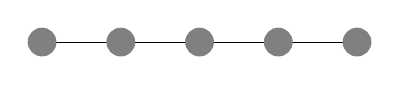
\begin{tikzpicture}

\draw (0,0) -- (4,0);
\filldraw [gray] (0,0) circle (5pt) [gray] (1,0) circle (5pt) [gray] (2,0) circle (5pt) [gray] (3,0) circle (5pt) [gray] (4,0) circle (5pt);
\end{tikzpicture}

\tikz \draw (0,0) node{1} (1,0) node{2} (2,0) node{3} (3,0) node{4} (4,0) node{5};


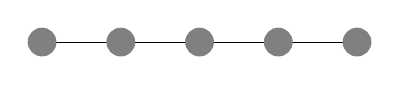
\begin{tikzpicture}

\draw (0,0) -- (4,0);
\filldraw [gray] (0,0) circle (5pt) [gray] (1,0) circle (5pt) [gray] (2,0) circle (5pt) [gray] (3,0) circle (5pt) [gray] (4,0) circle (5pt);


\end{tikzpicture}
% \end{center}

\section{Distância entre duas permutações}

A distância de reversão entre $\pi$ e $\rho$ denotada por $d(\pi,\rho)$ é o menor inteiro $k$ tal que existem permutações $\alpha_1,\ldots,\alpha_k$ tal que $\pi \ \circ \ \alpha_1 \ \circ \ \alpha_2 \ \circ \ \ldots \ \circ \ \alpha_k = \rho$. O problema da \textbf{distância de reversão} é: dadas duas permutações quaisquer $\pi$ e $\rho$, determinar $d(\pi,\rho)$. A distância $d$ é uma métrica \cite{Lages} e medir a distância de reversão entre uma permutação $\pi$ qualquer e $\iota$ é calcular a distância da \textbf{ordenação} de $\pi$, denotada por $d(\pi,\iota) = d(\pi)$.
% Assim a distância entre $\pi$ e $\rho$, $d(\pi, \rho) = k$ onde $k$ denota essa quantidade miníma de reversões. Como distância, $d$  satisfaz os axiomas de métrica provados por , mas neste texto omitimos a demonstração destas propriedades.
% \FV{$d$ é uma função? Ou um número?}
% , ou seja, a quantidade de evolução a nível cromossômico que procede as reversões.
% Seja $\pi$ uma permutação qualquer, tal que:

% \[\pi = (\pi_1 \ \ 
% \pi_2 \ \ 
% \pi_3 \ \ 
% \pi_4 \ \ \ldots \ \ 
% \pi_n) \ \ \]
% \begin{itemize}
%     \item $d(\pi_i, \pi_i) = 0$. \\A distância entre um elemento $\pi_i$ e ele mesmo é sempre 0.
%     \item $Se \ \pi_i \neq \pi_j, \ logo      \ d(\pi_i, \pi_j) > 0$. \\A distância entre quaisquer dois elementos distintos de $\pi$ sempre será maior que 0.
%     \item $d(\pi_i, \pi_j) = d(\pi_j, \pi_i)$.
%     \item $d(\pi_i, \pi_k) \leq d(\pi_i, \pi_j) + d(\pi_j, \pi_k)$.
% \end{itemize}

% \FV{Por que ``lema'' (abaixo)?}
\begin{prop}
Calcular a distância de reversões entre as permutações $\pi$ e $\rho$ é equivalente a calcular a distância de ordenação da permutação $\pi^{-1} \circ \rho$.
\end{prop}
\begin{prova}
% Suponha que encontrar a distância de reversão entre as permutações $\pi$ e $\rho$ é equivalente a encontrar a distância de reversão de $\pi^{-1} \circ \rho$ e a permutação identidade $\iota$. Desta forma, podemos reescrever como, $\tau = \pi^{-1} \circ \rho $ e computar a distância de $\tau$  e $\iota$. Esta formulação do problema de distância passa a ser um problema de \textbf{Ordenação por reversões}, ou seja estamos generalizando o problema de distância de reversões de modo que para toda instância do problema o objetivo seja ordenar a permutação.
Sendo $\alpha_i$ uma reversão $[i, j]$, suponha que $\alpha_1, \alpha_2 \ \ldots,\alpha_k$ é uma sequência de reversões que transforma $\pi$ em $\rho$, ou seja:
\[ \pi \ \circ \ \alpha_1 \ \circ \ \alpha_2 \ \circ \ \ldots \ \circ \ \alpha_k = \rho\]

% Adicionando $\pi^{-1}$ e $\alpha_{k} \circ \alpha_{k-1} \ldots \alpha_1$ aos dois lados da equivalência, temos que: \\

Adicionando $\pi^{-1}$ aos dois lados da equivalência, temos que: \\
% \[\textcolor{blue}{\pi^{-1}} \circ \pi \circ \alpha_1 \circ \ldots\alpha_k \circ \textcolor{blue}{\alpha_{k} \circ \alpha_{k-1} \ldots \alpha_1 = \pi^{-1}} \circ \rho \circ \textcolor{blue}{\alpha_{k} \circ \alpha_{k-1} \ldots \alpha_1}\]


\[ \underbrace{\pi^{-1}} \circ \ \pi \circ \alpha_1 \circ \ldots\alpha_k \circ = \underbrace{\pi^{-1}} \circ \rho \]
\begin{center}
$\downarrow$
\end{center}
\[ \underbrace{\pi^{-1} \circ \pi}_{\iota} \circ \ \alpha_1 \circ \ldots  \alpha_k = \pi^{-1} \circ \rho \]

Adicionando $\alpha_{k} \circ \alpha_{k-1} \ldots \alpha_1$ aos dois lados da equivalência, temos que:

\[ \iota \circ \alpha_1 \circ \ldots\alpha_k \circ \underbrace{\alpha_{k} \circ \alpha_{k-1} \ldots \alpha_1} = \pi^{-1} \circ \rho \circ \underbrace{\alpha_{k} \circ \alpha_{k-1} \ldots \alpha_1}\]



Pela Propriedade \ref{prop2} segue que:\\
\[ \iota \circ \underbrace{\alpha_1 \circ \ldots \underbrace{\alpha_k \circ \alpha_{k}}_{\iota} \circ \alpha_{k-1} \ldots \alpha_1}_{\iota} = \pi^{-1} \circ \rho \circ \underbrace{\alpha_{k} \circ \alpha_{k-1} \ldots \alpha_1}\]

\begin{center}
$\downarrow$
\end{center}

\[ \iota = \pi^{-1} \circ \rho \circ \alpha_{k} \circ \alpha_{k-1} \ldots \alpha_1\]
% \[\pi^{-1} \circ \pi \circ \alpha_1,\alpha_2, \ldots,\alpha_k \alpha_{k} \circ \alpha_{k-1} \ldots \alpha_1 = \iota\]
Logo:
\begin{center}
${\alpha_{k} \circ \alpha_{k-1} \ldots \alpha_1}$ transforma $\pi^{-1} \circ \rho$ em $\iota$
\end{center} 
\end{prova}

Com isso, o problema de distância de reversão passa a ser um problema de \textbf{Ordenação por reversões}, ou seja estamos generalizando o problema de distância de reversões de modo que para toda instância do problema o objetivo seja ordenar a permutação.

% uma das permutações se torne sempre a identidade $\iota$, assim nosso objetivo passa ser o de sempre ordenar a permutação de entrada de modo a alcançar a permutação identidade.

% O impacto disso em nossos experimentos e estudos é que sendo um problema de ordenação, nossa permutação objetivo sempre será a permutação identidade.

\section{\textit{Breakpoints} e adjacências}
%Colocar a notacao de elementos adjacentes

 Um \textbf{\textit{breakpoint}} (BP) de uma permutação $\pi$ é um par de elementos $\pi_i, \pi_{i+1}$, tal que $|\pi_{i+1} - \pi_i| \neq 1$. Quando $|\pi_{i+1} - \pi_i| = 1$, chamamos esse par de \textbf{adjacência}, ou seja $\pi_i$ é adjacente a $\pi_{i+1}$ e denotamos por $\pi_{i+1}$ $\sim$ $\pi_i$. Com o intuito de lidar com \textit{breakpoints} nas extremidades das permutações em nossas implementações os elementos $\pi_0 = 0$ e $\pi_{n+1} = n+1$ são adicionados para destacar os BP formados por elementos nas extremidades da permutação, essa mudança não fere a definição anterior pois não aumenta a quantidade de BP da permutação. Assim, garantimos que os elementos das extremidades da permutação estão na posição correta pois temos um referencial para ordenar os demais elementos internos. A quantidade de \textit{breakpoints} em uma permutação $\pi$ é denotada por $\phi(\pi)$ (lê-se fi de pi) e a diferença da quantidade de \textit{breakpoints} entre uma permutação qualquer $\pi$ e uma reversão $\rho$ aplicada a ela é  denotada por $\Delta \phi(\pi)$ (lê-se delta fi), assim $\Delta \phi(\pi) = \phi(\pi) - \phi (\pi \circ \rho)$. Os valores para  $\Delta \phi(\pi)$ sempre estão entre $-2$ e $2$, pois uma única reversão não pode eliminar ou aumentar mais do que 2 \textit{breakpoints} na permutação.
 
Definimos como \textit{strip} de uma permutação $\pi$ um intervalo de elementos $i, j$, $i \leq j$ tal que os elementos nas posições $(i-1, i)$ e $(j,j+1)$ são BP e que não existam BP nos elementos dentro do intervalo. Sendo assim, todos elementos dentro do intervalo são adjacentes. Além disso, caso esses elementos estejam em ordem crescente, dizemos que essa é uma \textit{strip} crescente (SC). Caso contrário, ela será \textit{strip} decrescente (SD). Os elementos $\pi_0$ e $\pi_{n+1}$ inseridos por nós sempre estarão em uma SC.
% Definimos como \textit{strip}
% crescente (SC) como uma faixa de elementos em ordem crescente na permutação, e definimos como \textit{strip} decrescente uma faixa de elementos em ordem crescente na permutação. Essas duas definições nos servem como base para alguns lemas que veremos mais adiante, e nos ajudam a fundamentar o funcionamento dos algoritmos.

\section{Limitantes}
Nesta seção descreveremos os limitantes inferior e superior para $d(\pi)$, ou seja, os limites do quão boas nossas soluções podem ser,
% , considerando os casos mais favoráveis e os mais desfavoráveis.  .
% Para nosso trabalho, assim como \cite{kececioglu1995exact}, uma parte fundamental é entender como é comportamento das metodologias aplicadas para a obtenção das soluções. Dado isso, esta seção descreve dois pontos que usamos como partida para a construção de nossas soluções, eles estão ligados aos algoritmos usados como 

\subsection{Algoritmo Ingênuo -  Limitante Superior}
\label{algoritmo_ingenuo}
O algoritmo ingênuo é uma das maneiras de se obter um limitante superior para o problema de ordenação por reversões. Os passos do algoritmo ingênuo são: faça uma reversão que coloque o elemento $1$ na primeira posição caso ele já não esteja na primeira posição, após isso faça o mesmo para o elemento $2$, repita este processo até que o elemento $n-1$ fique na $(n-1)$-ésima posição da permutação. No pior dos casos, será necessário fazer $n - 1$ reversões. Assim podemos garantir que qualquer permutação será ordenada em no máximo $n - 1$ reversões, e este é o nosso limitante superior, nenhuma outra solução que gaste mais reversões do que esta nos será relevante, ou seja, $d(\pi) \leq n-1$ para qualquer $\pi \in S_n$.


\subsection{Limitante Inferior}
\label{limitante inferior}
Uma das maneiras de se obter um limitante inferior é pela propriedade de remover BP da uma permutação. Ordenar uma permutação é remover todos BP contidos nela, visto que uma reversão afeta apenas duas extremidades de um intervalo de elementos (\textit{endpoints}), o máximo de BP que conseguimos remover com uma única reversão é dois BP no melhor cenário. Podemos generalizar isso para todos os BP de uma permutação, assim nosso limitante inferior será $(\phi(\pi))/2$. Desta forma nosso limitante traduz-se em ordenar a permutação com uma quantidade de reversões que seja a metade da quantidade de BP na permutação pois supomos que cada reversão remove 2BP, existem outras soluções melhores mas para nossos experimentos esse foi o limitante adotado.


\section{Permutações de Gollan}
% \FV{Que notação é essa: $d(n)$?}
A permutação de Gollan $G_n$ é uma permutação que possui uma propriedade especial: $d(G_n) = n - 1$ \cite{kececioglu1995exact}, isto é, requer $n-1$ reversões para ser ordenada. Somente $G_n$ e $G_n^{-1}$ possuem esta propriedade. Para construir uma permutação de Gollan, utilizamos a seguinte regra: 
% \FV{Definição abaixo em inglês?}
% \RR{DEFINIR d()}
\[G_{n+1} \ = \ \left \{
\begin{array}{cl}
  (1), & n \ \mbox{é zero}; \\
   (G_n(1) \ \ G_n(2) \ \ \ldots \ \ (G_n(n-1) \ \ n+1 \ \ G_n(n)),& n \ \mbox{é  ímpar}; \\
    ( G_n(1) \ \ G_n(2) \ \ \ldots \ \ (G_n(n-2) \ \ n+1 \ \ G_n(n) \ \ G_n(n-1)),& n \ \mbox{é par};
\end{array}
\right.\]

A permutação de Gollan tem importância fundamental em nossos experimentos na Seção \ref{cap:experimentos}, pois dado que $d(\pi) \leq n-1$ para todo $\pi \in S_n.\ G_n$ necessita da maior quantidade de reversões para ser ordenada, sendo este um ponto chave para nossas avaliações de desempenho através dos testes executados.

% A permutação de Gollan tem importância fundamental em nossos experimentos na \textbf{Seção 5}, pois por ser a permutação que necessita da maior quantidade de reversões para ser ordenada, consequentemente ela também é a que exige o maior esforço por parte dos algoritmos e das técnicas implementadas, sendo este um ponto chave para nossas avaliações de desempenho através de testes de estresse.

% \begin{figure}[h]
% \caption{Geração de uma PG}

% \centering % para centralizarmos a figura
% 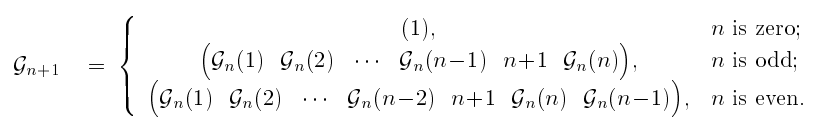
\includegraphics[width=15cm]{Imagens/Gollan.png} % leia abaixo
% \label{figura:Gollan}
% \end{figure}

% \section{Nosso Problema}
% As raízes de nosso problema de distância de reversão vem do problema de \textbf{\textit{edit distance}}, um problema da computação que consiste em 
% encontrar o menor conjunto de operações necessárias para transformar uma \textit{string} em outra.
% \section{Lemas, Teoremas e Corolários}

% \section{Propriedades}

% Algumas propriedades foram extraídas de \cite{kececioglu1995exact} e acompanham nosso processo de compreensão do problema de ordenação por reversões.

% \begin{lema}
% \label{lema1}
%  Toda permutação $\pi$ com uma subcadeia decrescente (SD) possui uma reversão que remove um \textit{breakpoint}.
% \end{lema}
% \begin{prova}
% Seja $x$ o menor elemento em uma subcadeia 
% decrescente em $\pi$ e $i$ o inteiro tal que $\pi_i = x$. Note que $x \ge 1$ pois 0 está em uma subcadeia crescente e $(\pi_i, \pi_{i+1})$ formam um breakpoint. Além disso, $x-1$ está em uma subcadeia crescente. Logo $x-1 \ge 0$ e portanto é um elemento de $\pi$. Seja $j$ o inteiro tal que $\pi_j = x-1$.
% Então, ou $i < j$ ou $i > j$.

% Suponha que $i < j$. Suponha que $(\pi_{j_1}, \pi_j)$ seja um breakpoint, então $(\pi_j, \pi_{j+1})$ é uma adjacência senão $\pi_j$ sozinho seria uma subcadeia decrescente contrariando a minimalidade de $x$. Logo 
% $\pi_{j+1} = x-2$ o que implica novamente que 
% $\pi_j$ está em uma subcadeia decrescente contrariando novamente a escolha de $x$.
% Logo, assumimos que $(\pi_{j-1}, \pi_j)$
% é uma adjacência, ou seja, $\pi_{j-1} = x -2$. Portanto, $(\pi_j, \pi_{j+1})$ é um breakpointo. Logo a reversão $[i,j]$ remove pelo menos um BP.
% \end{prova}

% \FV{O que é ``Lema em passo a passo''?}

% \textbf{Lema em passo a passo:}
% \begin{enumerate}

%     \item $\pi$ possui um SD: escolha o SD aquele que possui o menor elemento $\pi_i$, digamos \[
%     |\ldots  8 \ 7 \ 6 \ 5 |.\]
   
%     \item Todos os números menores que $\pi_i = 5$ estarão em uma SC, pois se não $\pi_i$, não seria o minimal. \[
%     |1 \ 2 \ 3 \ 4 | 8 \ 7 \ 6 \ 5 |.\]
   
%     \item Existe um único \textit{breakpoint} na permutação $\pi$ \[
%     [1 \ 2 \ 3 \underbrace{4 | 8} \ 7 \ 6 \ 5 ].\]
    
%     \item Aplicando uma reversão sobre a SD conseguimos ilustrar que existe uma reversão que remove uma BP
%     \[ [1 \ 2 \ 3 \ 4 \underbrace{8 \ 7 \ 6 \ 5} ].\]
%     \[ [1 \ 2 \ 3 \ 4 \ 5 \ 6 \ 7 \ 8 ].\]

% \end{enumerate}

% \begin{lema}
% \label{lema2}
%  Seja $\pi$ uma permutação com uma SD. Se toda reversão que remove 1 BP de $\pi$ deixa a permutação sem SD, $\pi$ possui uma reversão que remove 2 BP.

% \end{lema}
% \begin{prova}
% Considerando uma SD de $\pi$ contendo o menor elemento $\pi_i$. Portanto a SC que contém $\pi_i-1$ deve estar a esquerda da subcadeia que contém $\pi_i$.
% Considerando a SD de $\pi$ da qual o primeiro elemento, $\pi_j$ é o maior. O elemento $\pi_j+1$ deve estar em uma SC (do contrário $\pi_j$ não é o maior) a direita da subcadeia que contém $\pi_j$
% \end{prova}
% \begin{enumerate}
%      \item $\pi$ possui um SD que possui o menor elemento $\pi_i$, digamos \[
%     \ldots |4 \ 3 \ 2 | \ldots \]
%     \item Portanto a SC que contém $\pi_{i-1}$, deve estar a esquerda da \textit{strip} contendo $\pi_i$ \[
%     \ldots |1 \ 5 \ 6 \ | \ldots | 4 \ 3 \ 2 | \ldots.\]
%     \item $\pi$ possui uma SD que possui o maior elemento $\pi_j$, digamos.
%     \[\ldots |10 \ 8 \ 6 | \ldots \]
%     \item Portanto a SC que contem $\pi_{j+1}$ deve estar a direita da \textit{strip} contendo $\pi_j$
%     \[
%     \ldots |10 \ 8 \ 7 \ | \ldots | 9 \ 11 \ 12 | \ldots.\]
    
    
 
% \end{enumerate}



% \begin{lema}
% \label{lema2}
% Para toda permutação $\pi$, aplicar reversões aleatórias em $\pi$ (ou seja, embaralhar os elementos) aumentará a quantidade de reversões para ordená-la até um determinado ponto.
% \end{lema}

% \begin{prova}
% Seja $\pi_n$ com $n \in \mathbb{N}$, a menor quantidade de BP que $\pi$ pode possuir é 0-BP, ou seja $\pi = \iota$. Reversões aleatórias podem aumentar a quantidade de BP em $\pi$, tirando elementos da posição correta, entretanto o máximo de BP que $\pi$ pode possuir é $(n-1)BP$, a quantidade de BP é limitada pelo próprio tamanho da permutação, ou seja, continuar embaralhando a permutação não aumentará a quantidade de BP, consequentemente a quantidade de reversões necessárias para ordenação também não aumentará. 
% \end{prova}

% aumentar a quantidade miníma necessária de reversões para se ordenar a permutação sem aumentar a quantidade de elementos da permutação só é possível até um determinado ponto.


% \FV{De novo, uma enumeração abaixo}
% \textbf{Lema em passo a passo:}

% \begin{enumerate}
%     \item O mínimo de \textit{breakpoints} que uma permutação sobre $n$ pode ter é 0 BP, ou seja é a permutação identidade.
%     \item O máximo de breakpoints que uma permutação $\pi$ qualquer sobre $n$ pode ter é $n-1$ BP.
%     \item A partir de uma permutação identidade podemos aplicar múltiplos embaralhamentos que aumentem a sua quantidade de BP, consequentemente aumentam a quantidade de reversões necessárias para a ordenação.
%     \item Porém, a quantidade de BP $\phi(\pi)$ é limitada por $n-1$, não sendo possível aumentar essa quantidade apenas embaralhando a permutação, sem modificar o valor de $n$.
%     \item Logo, podemos garantir que há um limite do quanto é possível aumentar a "dificuldade" de se ordenar uma permutação (onde aumentar a dificuldade traduz-se como aumentar a quantidade de reversões necessárias para ordenar) com base em sua quantidade de elementos. Com isso a partir de determinado ponto esta dificuldade torna-se independente da quantidade de embaralhamento aplicado à permutação, 
% \end{enumerate}

 \section{Permutações de teste}

 Além das permutações de Gollan, outras permutações foram utilizadas nos experimentos descritos na Seção~\ref{cap:experimentos}, construídas a partir de um pré-processamento. A primeira classe de permutações criada foi a de permutações aleatórias (PR). Neste caso, iniciamos a partir de permutações identidade de tamanhos variados e utilizamos o método \textit{shuffle}() da biblioteca \textit{random} da linguagem Python. Este método embaralha os elementos da permutação criando assim uma permutação aleatória.  
  \[ \iota = (1 \ 2 \ 3 \ 4  \ \ldots \ n) \rightarrow \textit{shuffle}(\iota) \rightarrow (\pi_1 \ \pi_2 \ \pi_3 \ \ldots \ \pi_n)=\pi \neq \iota.\]
 
 A segunda classe de permutações que criamos são as permutações geradas por reversões aleatórias (PGR), iniciando com uma permutação identidade e escolhendo aleatoriamente dois números inteiros $i, j$ tais que  $1 \leq i \leq j \leq n$, utilizando o método \textit{randint}(). Aplicamos uma reversão $[i, j]$, a qual chamamos de reversão de embaralhamento (o seu oposto seria uma reversão de ordenação). Repetimos esse processo inúmeras vezes, utilizando diferentes valores $i, j$, ao fim temos uma permutação gerada por reversões aleatórias:
 
    % \[\iota = (1 \ 2 \ 3 \ 4  \ \ldots \ n)\]
    \[\iota \ \circ \ [i, j] \ \circ \ [i, j] \ \circ \ [i, j] \ \circ \ldots \ \circ \ [i, j] = \pi\]
    
 A partir dos experimentos com PGRs, fomos capazes de visualizar uma propriedade das permutações:

\begin{prop}
\label{prop4}
Aplicar reversões aleatórias em $\pi$ (ou seja, embaralhar os elementos) aumentará a quantidade de reversões para ordená-la até um determinado ponto.
\end{prop}
\begin{prova}
Seja $\pi_n$ com $n \in \mathbb{N}$, a menor quantidade de BP que $\pi$ pode possuir é 0-BP, ou seja $\pi = \iota$. Reversões aleatórias podem aumentar a quantidade de BP em $\pi$, tirando elementos da posição correta, entretanto o máximo de BP que $\pi$ pode possuir é $(n-1)$BP, a quantidade de BP é limitada pelo próprio tamanho da permutação, ou seja, continuar embaralhando a permutação não aumentará a quantidade de BP, consequentemente a quantidade de reversões necessárias para ordenação também não aumentará. 
\end{prova}
% Cada $\rho_i$ representa a reversão de um intervalo $[i, j]$.

% \FV{Não consigo entender o que você quis dizer acima. Além do mais, o valor de $n$ agora não é mais o comprimento da permutação?}







